El modelo atómico de Bohr es un modelo clásico del átomo propuesto en 1913 por el físico danés Niels Bohr, el cual explicaba que los electrones giran alrededor del núcleo del átomo en órbitas circulares específicas, y que solo pueden ocupar ciertos niveles de energía\cite{Bohr1913}.

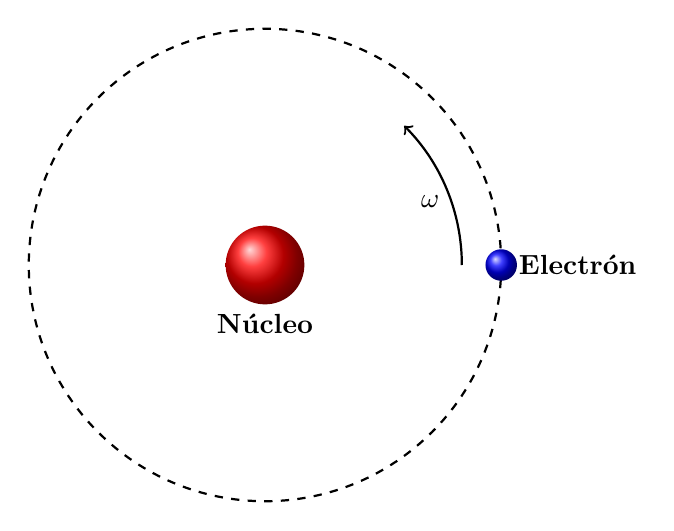
\begin{tikzpicture}
  % Nucleus
  \shade[ball color=red] (0,0) circle (0.5);
  \node[below] at (0,-0.5) {\textbf{Núcleo}};

  % Orbital
  \draw[thick,dashed] (0,0) circle (3);

  % Electron
  \shade[ball color=blue] (3,0) circle (0.2);
  \node[right] at (3.1,0) {\textbf{Electrón}};

  % Motion
  \draw[->,thick] (2.5,0) arc[start angle=0,end angle=45,radius=2.5];
  \node at (2.1,0.8) {$\omega$};
\end{tikzpicture}

En el modelo, el electron tiene la capacidad de pasar de una órbita a otra cuando absorbe o emite energía en forma de fotones. La energía que se le debe suministrar para subir al siguiente estado energético o de excitación es de un valor específico, del mismo modo, al trasladarse de un estado excitado al estado fundamental, este libera esa energía como radiación electromagnética.

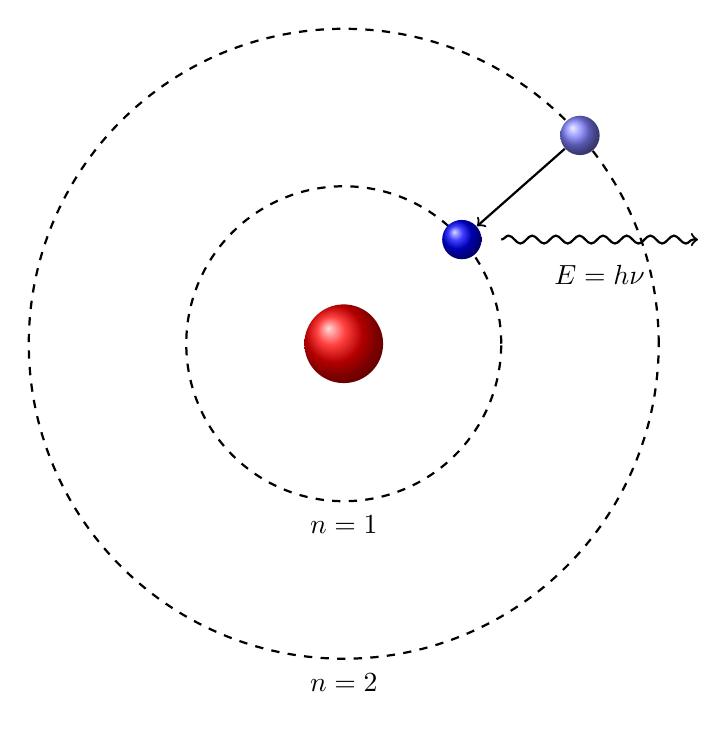
\begin{tikzpicture}

  % Nucleus
  \node[ball color=red, circle, minimum size=1cm] (nucleus) at (0,0) {};

  % Energy levels
  \draw[thick,dashed] (0,0) circle (2cm);
  \node at (0,-2.3) {\textbf{\(n = 1\)}};

  \draw[thick,dashed] (0,0) circle (4cm);
  \node at (0,-4.3) {\textbf{\(n = 2\)}};

  % Electrons
  \node[ball color=blue!50, circle, minimum size=0.5cm] (electron_outer) at (3,{sqrt(7)}) {};
  \node[ball color=blue, circle, minimum size=0.5cm] (electron_inner) at (1.5,{sqrt(1.75)}) {};

  % Electron transition
  \draw[->, thick] (electron_outer) -- (electron_inner);

  % Photon emission (wavy arrow)
  \draw[->, thick, decorate, decoration={snake, amplitude=0.5mm, segment length=3mm}] 
    (electron_inner) + (0.5,0) -- +(3,0) node[midway, below=0.2cm] {\( E = h\nu\)};

\end{tikzpicture}
Cada átomo emite frecuencias de luz características según su configuración electrónica, lo que da lugar a su espectro de emisión. Este espectro corresponde al conjunto de frecuencias de radiación electromagnética emitidas cuando un átomo realiza transiciones desde un estado excitado a uno de menor energía.

La energía de cada fotón emitido es igual a la diferencia de energía entre los estados involucrados. Dado que un átomo puede experimentar múltiples transiciones electrónicas, cada una con una diferencia de energía específica, estas transiciones producen un conjunto único de longitudes de onda que forman el espectro de emisión.

El espectro de emisión de un elemento es único y sirve para identificarlo. Por ello, se utiliza ampliamente en la identificación de elementos en materiales de composición desconocida y en el análisis químico de sustancias\cite{Kirchhoff1859}.

\begin{figure}[H]
    \centering
    
\includegraphics[width=1\linewidth]{Image/Emission_spectrum-H.png}
    \caption{Lineas de emisión del hidrogeno.}
    \label{fig:lines_H}
\end{figure}
\begin{figure}[H]
    \centering
    
\includegraphics[width=1\linewidth]{Image/Emission_spectrum-Na.png}
    \caption{Lineas de emisión del sodio.}
    \label{fig:lines_Na}
\end{figure}

Para identificar las lineas correspondientes se utiliza la ley de \textit{Fraunhoffer} que describe el fenómeno de la difracción en el régimen de campo lejano, es decir, cuando la distancia entre el objeto que causa la difracción (como una rendija o una red de difracción) y el punto de observación es considerablemente mayor que el tamaño de la apertura o del objeto que produce la difracción\cite{Fraunhofer1821}.

\begin{equation}
    n\lambda=d\sin{\theta}
\end{equation} 

En donde $n$ es el orden máximo de difracción, $\lambda$ es la longitud de onda incidente, $d$ es la separación en la red de difracción y $\theta$ es el ángulo de difracción máximo.

Del mismo modo que se puede identificar los elementos usando el espectro de emisión, también se puede hallar la constante de plank, aplicando la fórmula de \textit{Rydberg}

\begin{equation}\label{eq:formula_Rydberg}
    \frac{1}{\lambda}=R_{\infty}(\frac{1}{n'^2}-\frac{1}{n^2})
\end{equation}

La ecuación \ref{eq:formula_Rydberg} describe que el inverso de la longitud de onda respecto es igual a una constante denominada la constante de \textit{Rydberg} $R_{\infty}$ y al cambio en la órbita del electrón\cite{rydberg1914}.

La constante de \textit{Rydberg} tiene la equivalencia\cite{griffiths2017}.

\begin{equation}\label{Rydberg}
    R_{\infty}=\frac{me^4}{8\epsilon_0^2h^3c}
\end{equation}

En donde $m$ es la masa del electrón, $e$ es su carga, $\epsilon_0$ es la permitividad electrica del vacío y $c$ es la velocidad de la luz.
Aplicando la ecuación \ref{Rydberg} a \ref{eq:formula_Rydberg} y despejando $h^3$ se encuentra que

\begin{equation}\label{eq:planck}
  h^3 = \frac{e^4 m}{8 \epsilon^2_0 c}\left( \frac{1}{2^2} - \frac{1}{n^2_j} \right) \lambda
\end{equation}
